\documentclass[tikz,border=4pt]{standalone}
\usepackage[utf8]{inputenc}
\usepackage[T1]{fontenc}
\usepackage{helvet}
\renewcommand{\familydefault}{\sfdefault}
\usetikzlibrary{arrows.meta,shapes.geometric,positioning}
\begin{document}
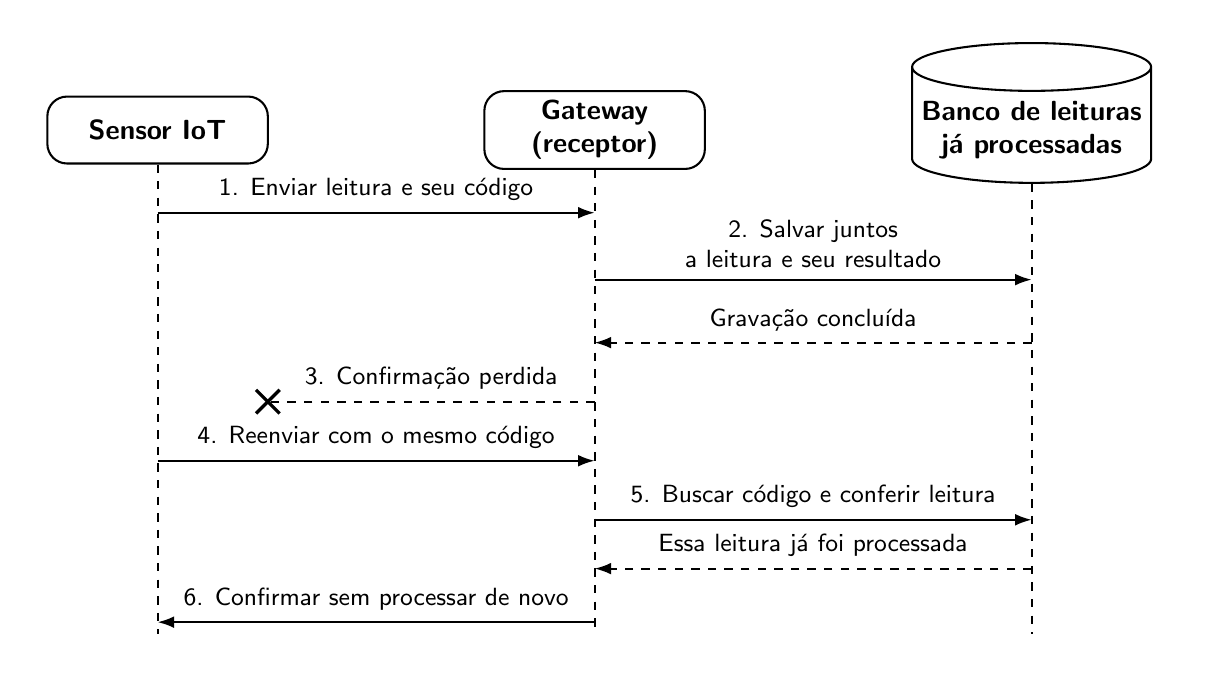
\begin{tikzpicture}[
  font=\sffamily\fontsize{10}{12}\selectfont,
  line width=0.75pt,
  flow/.style={-{Latex[length=2.1mm,width=1.5mm]}},
  message/.style={font=\sffamily\fontsize{9}{11}\selectfont,align=center,fill=white,inner sep=2pt},
  endpoint/.style={draw=black,fill=white,rounded corners=2.5mm,
    minimum width=2.8cm,minimum height=0.85cm,align=center,font=\bfseries}
]
\path[use as bounding box] (0,-0.35) rectangle (14.6,7.55);

\node[endpoint] (sensor) at (1.65,6.25) {Sensor IoT};
\node[endpoint] (gateway) at (7.20,6.25) {Gateway\\(receptor)};
\node[draw=black,fill=white,cylinder,shape border rotate=90,aspect=0.20,
  minimum width=2.8cm,minimum height=1.05cm,align=center,font=\bfseries]
  (ledger) at (12.75,6.25) {Banco de leituras\\já processadas};

\draw[dashed] (sensor.south) -- (1.65,-0.15);
\draw[dashed] (gateway.south) -- (7.20,-0.15);
\draw[dashed] (ledger.south) -- (12.75,-0.15);

\draw[flow] (1.65,5.20) -- node[message,above=2pt]
  {1. Enviar leitura e seu código} (7.20,5.20);
\draw[flow] (7.20,4.35) -- node[message,above=2pt]
  {2. Salvar juntos\\a leitura e seu resultado} (12.75,4.35);
\draw[flow,dashed] (12.75,3.55) -- node[message,above=2pt]
  {Gravação concluída} (7.20,3.55);

\draw[dashed] (7.20,2.80) -- node[message,above=2pt]
  {3. Confirmação perdida} (3.05,2.80);
\draw[line width=1.2pt] (2.90,2.65) -- (3.20,2.95);
\draw[line width=1.2pt] (2.90,2.95) -- (3.20,2.65);

\draw[flow] (1.65,2.05) -- node[message,above=2pt]
  {4. Reenviar com o mesmo código} (7.20,2.05);
\draw[flow] (7.20,1.30) -- node[message,above=2pt]
  {5. Buscar código e conferir leitura} (12.75,1.30);
\draw[flow,dashed] (12.75,0.68) -- node[message,above=2pt]
  {Essa leitura já foi processada} (7.20,0.68);
\draw[flow] (7.20,0.00) -- node[message,above=2pt]
  {6. Confirmar sem processar de novo} (1.65,0.00);
\end{tikzpicture}
\end{document}
